%! TeX program = pdflatex
%! TeX options = -synctex=1 -interaction=nonstopmode -halt-on-error
% Elsevier (elsarticle) submission root for Biomedical Signal Processing and
% Control.  The manuscript prose remains modular under ../a_abstract through
% ../g_conclusion; do not move section content here.
%
% Single-column preprint layout with double spacing (review) and line numbers,
% as expected for peer review.  For a journal-like preview swap the options to
% [final,5p,times,twocolumn,number,sort&compress].
\documentclass[preprint,review,12pt,number,sort&compress]{elsarticle}

% Packages used by the modular manuscript (graphicx and natbib are loaded by
% elsarticle itself).
\usepackage[T1]{fontenc}
\usepackage{lmodern}
\usepackage{amsmath,amssymb,amsfonts}
\usepackage{booktabs}
\usepackage{array}
\usepackage{tabularx}
\usepackage{longtable}
\usepackage{float}
\usepackage{xurl}
\usepackage[hidelinks]{hyperref}
\usepackage{lineno}

% Paths are relative to this elsarticle folder.
\graphicspath{{../e_result/figures/}{../figures/}{../images/}}
\makeatletter
\def\input@path{{../}}
\makeatother

\journal{Biomedical Signal Processing and Control}

\begin{document}

\begin{frontmatter}

\title{Epoch-Aware Threshold Estimation for Blink Detection in Naturalistic Driving EEG}

% Rodney Petrus Balandong is first and corresponding author.
\author[ums]{Rodney Petrus Balandong\corref{cor1}}
\ead{balandong@ums.edu.my}
\author[utar]{Nur Syahirah Roslan}
\author[cisir]{Syaimaa' Solehah Mohd Radzi}
\author[cisir]{Muhamad Hafiz Abd Latif}
\author[cisir]{Tong Boon Tang}

\cortext[cor1]{Corresponding author.}

\affiliation[ums]{organization={Faculty of Science and Natural Resources, Universiti Malaysia Sabah},
            city={Kota Kinabalu},
            postcode={88400},
            state={Sabah},
            country={Malaysia}}

\affiliation[utar]{organization={Department of Information Systems, Faculty of Information and Communication Technology, Universiti Tunku Abdul Rahman},
    state={Perak},
    country={Malaysia}}

\affiliation[cisir]{organization={Centre for Intelligent Signal and Imaging Research (CISIR), Electrical and Electronics Engineering, Universiti Teknologi PETRONAS},
            city={Seri Iskandar},
            postcode={32610},
            state={Perak},
            country={Malaysia}}




\begin{abstract}
In fatigue-driving studies, blink activity within the electroencephalography (EEG) is treated as marker of driver fatigue rather than noise. Thresholding is one of the most straightforward and widely used approaches for detecting blink activity from EEG signals. However, current approaches that use thresholding estimate a single amplitude threshold from a pool of blink-heavy and blink-free epochs concatenated together, which dilutes the amplitude statistics used for threshold estimation. This study presents an epoch-aware, three-stage pipeline that avoids this dilution by keeping blink-heavy and blink-free epochs separate when estimating the detection threshold. The three-stage pipeline first screened non-overlapping epochs by peak-to-peak amplitude, then estimated a sample-level threshold from the suspicious-epoch pool, and finally extracted blink regions and mapped them to epoch-local coordinates. The proposed pipeline and two established continuous-signal baselines were compared on the complete 32-channel montage using two naturalistic driving-EEG corpora, an internally collected dataset and  public dataset, evaluated with event-level overlap matching and macro-averaged $F_1$. Evaluated on this 32-channel montage configuration, the proposed pipeline reached macro-$F_1$ scores of 88.25\% on Internal and 80.68\% on public dataset, significantly exceeding both baselines on both corpora after Bonferroni-corrected Wilcoxon signed-rank tests. These results indicate that epoch-aware threshold estimation yields more reliable blink detection than continuous-signal thresholding in naturalistic EEG driving recordings.
\end{abstract}


% Research highlights: 3--5 bullets, each at most 85 characters incl. spaces.
% BSPC also requires these as a separate editable file (highlights.tex).
\begin{highlights}
\item Epoch-aware pipeline keeps blink-heavy and blink-free EEG epochs apart
\item Threshold is estimated from a peak-to-peak screened suspicious-epoch pool
\item Evaluated on two naturalistic driving-EEG corpora with 32-channel montage
\item Macro-F1 of 88.25\% (Internal) and 80.68\% (public) beat both baselines
\item Gains are significant under Bonferroni-corrected Wilcoxon signed-rank tests
\end{highlights}

% Graphical abstract is encouraged but optional; submit it as a separate file
% (531 x 1328 px or larger; TIFF, EPS, PDF or MS Office).
%\begin{graphicalabstract}
%\includegraphics{grabs}
%\end{graphicalabstract}

\begin{keyword}
blink detection \sep electroencephalography \sep fatigue \sep
driving \sep threshold selection
\end{keyword}

\end{frontmatter}

\linenumbers

% The introduction follows a paragraph-per-file structure (one paragraph, one
% file) as required by instruction_agentic/rule/latex_writing_rule.md.
\section{Introduction}

\input{b_intro/p001/paragraph}

\input{b_intro/p002/paragraph}

%\input{b_intro/p003/paragraph}

%\input{b_intro/p004/paragraph}
\input{b_intro/p004/paragraph_compress}

\input{b_intro/p005/paragraph}

%\input{b_intro/p006/paragraph}

\input{b_intro/p007/paragraph}
\input{b_intro/p008/paragraph}
%
\section{Related Work}
%file:///C:/Users/balan/Downloads/peerj-cs-3249.pdf

%However, most of these methods require empirically preset  conditions, and few have explored whether the boundaries of blink artifact intervals are  accurately recognized. Amplitude thresholding, which is based on a priori estimation of  blink artifact amplitude, achieves the detection of blink peaks and thus blink position  localization

% add also study by https://www.sciencedirect.com/science/article/pii/S0165027010003894?via%3Dihub:Currently, the primary methods to detect blink artifacts involve amplitude thresholding
%(Nolan, Whelan & Reilly, 2010),
The classical literature established the difficulty of ocular contamination and motivated automated statistical detection directly from EEG. Early work emphasized artifact removal and statistical screening rather than blink-region benchmarking per se, but it already showed that extreme-value behavior, channel context, and morphology matter \citep{croft2000removal,klein2013reliable}. This historical backdrop explains why simple one-value global thresholds can be attractive, yet brittle.

A first important stream comprises single-channel or few-channel threshold-centered detectors. Chang et al.~\citep{chang2016detection} detect blink artifacts from a single prefrontal channel using digital filtering and rule-based decisions. Tran et al.~\citep{tran2021detection} present an explicitly thresholding-based EEG blink detector and compute a minimum amplitude threshold from transformed signal magnitude and signal standard deviation. Zhang et al.~\citep{zhang2023method} move toward real-time frontal EEG detection with short windows and decision logic around potential blink boundaries. Wang et al.~\citep{wang2022multidimensional} extend thresholding to harder clinical settings by optimizing multidimensional features in the presence of epileptiform discharges, and later work based on higher-order cumulants continues the move toward short-segment single-channel detection \citep{wang2025sliding}.

A second stream contains hybrid thresholding pipelines. BLINKER first identifies candidate intervals with a mean-based standard-deviation threshold and then rejects implausible candidates using robust amplitude-distribution criteria derived from the median absolute deviation \citep{kleifges2017blinker}. Cao et al.~\citep{cao2021unsupervised} use cascaded thresholding over amplitude, amplitude displacement, and cross-channel correlation before applying a Gaussian mixture model. Agarwal et al.~\citep{agarwal2019blink} self-learn user-specific profiles in an unsupervised manner, while Valderrama et al.~\citep{valderrama2018automatic} use iterative template matching and automatic threshold/template estimation for suppression in single-channel recordings. Guttmann et al.~\citep{guttmann2019new} further emphasize adaptation to inter- and intra-subject variability, underscoring that fixed thresholds are often not enough.





%Therefore, it is necessary to establish an assumption-free detection approach capable of  adaptively and more precisely identifying blink artifacts of varying durations by exploiting  the inherent characteristic distinctions between EEG signals and blink artifacts.

%A growing stream of blink and ocular-artifact research replaces hand-tuned thresholds with data-driven models. Convolutional neural networks have been used both to detect eye-blink artifacts and to remove them from EEG~\citep{jurczak2022implementation,gawande2022deep}, while transformer- and video-based architectures have pushed blink-detection accuracy further~\citep{fodor2023blinklinmult,hong2024robust}. Autoencoder and segmentation-denoising networks also target single-channel artifact removal~\citep{faisal2025eye,li2023segmentation}, and recent reviews catalogue the broader shift from conventional thresholding toward deep learning for physiological-artifact handling, including in wearable EEG~\citep{akshathraj2026physiological,arpaia2025systematic}. In driving and fatigue monitoring, machine-learning and CNN models detect drowsiness from blink and eye-state cues~\citep{cabot2024drowsiness,makhmudov2024real}. These data-driven detectors can be accurate, but they typically require labelled training data, more computation, and offer less transparency than a single interpretable threshold. This contrast motivates studying the lightweight thresholding stage itself, which frequently precedes or complements such pipelines, and in particular the epoch-structure estimation bias that this paper addresses.

\section{METHOD AND MATERIALS}\label{sec:method}
%\input{d_method/m_pipeline_overview}
%
%
%\input{d_method/step1_select_bad_epoch}
%\input{d_method/step2_get_threshold_candidates}
%\input{d_method/step3_get_blink_regions}

\input{d_method/experiment_setup}
\section{Results}
\label{sec:results}



% =====================================================================
% EXPERIMENT 1 — channel selection
% =====================================================================
\subsection{Experiment 1: EEG Channel-Subset Analysis}
\label{sec:exp1_channel}
\input{e_result/exp1/sec}


% =====================================================================
% EXPERIMENT 2 — epoch duration
% =====================================================================
\subsection{Experiment 2: Stability Across Epoch Durations}
\label{sec:exp3_epoch}

\input{e_result/exp2/sec}



% NOTE (commented out on purpose, do not delete): this ablation ("Effect of the Threshold
% Estimator at Stage B") was archived to e_result/obs/exp3/sec.tex since it is not part of
% the active flow. Re-enable by moving that folder back and uncommenting here; see
% e_result/obs/README.md.
% \subsection{Effect of the Threshold Estimator at Stage B}
% \label{sec:estimator}
% \input{e_result/obs/exp3/sec}




% =====================================================================
% EXPERIMENT 3 — strategy comparison
% =====================================================================
\subsection{Experiment 3: Strategy Comparison}
\label{sec:exp3_strategy}
\input{e_result/exp3/sec}

%\subsection{Operating Points}
%\label{sec:operating_points}

%\begin{figure}[ht]
%    \centering
%    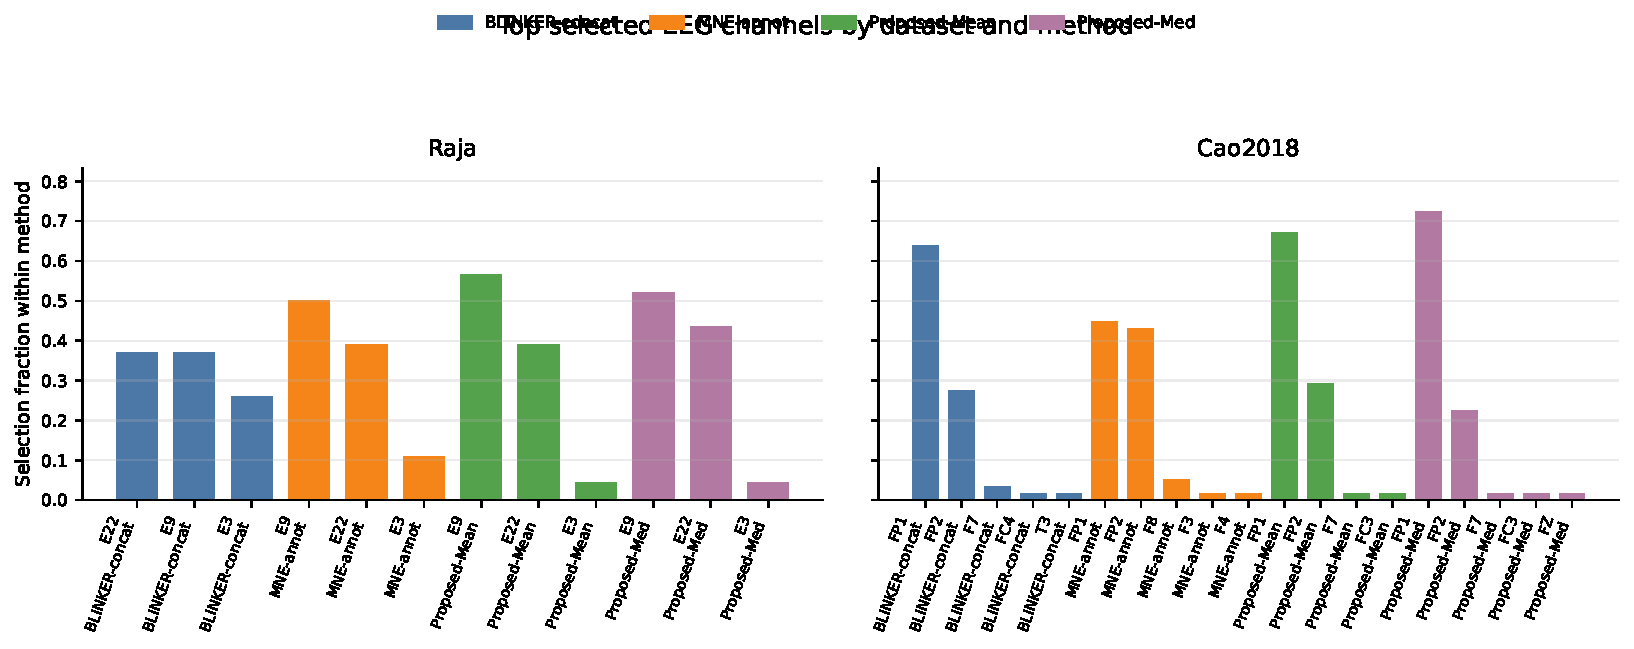
\includegraphics[width=0.9\linewidth]{fig_channel_selection.pdf}
%    \caption{Best-channel selection frequency, pooled over the four conditions.}
%    \label{fig:channel_selection}
%\end{figure}


\section{Discussion}
\label{sec:discussion}

\input{f_discussion/d1_frontopolar/par1}

% NOTE (commented out on purpose, do not delete): obs/d5_channel_instability drew its
% selection-frequency and cross-condition-agreement numbers from the "Stability of the
% Channel Choice" subsubsection (tab_channel_selection, p10_selection_frequency,
% p12_agreement), which is itself commented out of e_result/exp1/sec.tex. Re-enable this
% paragraph only alongside re-enabling that results subsection (move the folder back out
% of obs/ first; see f_discussion/obs/README.md).
%\input{f_discussion/obs/d5_channel_instability/paragraph}

\input{f_discussion/d2_epoch_stability/paragraph}

% NOTE (commented out on purpose, do not delete): obs/d3_estimator discusses the Stage-B
% median/MAD vs. mean threshold-estimator comparison, whose entire results subsection
% ("Experiment 3: Effect of the Threshold Estimator at Stage B", e_result/obs/exp3/sec.tex)
% is archived out of e_result/result.tex. Re-enable this paragraph only alongside
% re-enabling that results subsection (move the folder back out of obs/ first; see
% f_discussion/obs/README.md).
%\input{f_discussion/obs/d3_estimator/paragraph}

% NOTE: Experiment 3 is discussed in a single paragraph. d3_main_implication now also
% carries the precision-recall / threshold-dilution interpretation formerly in
% obs/d4_why_dilution (archived; see f_discussion/obs/README.md).
\input{f_discussion/d3_main_implication/paragraph}

\input{f_discussion/d5_limitations/paragraph}

\input{f_discussion/d6_future/paragraph}



\section{Conclusion}
\label{sec:conclusion}
\input{g_conclusion/p1}


% ---------------------------------------------------------------------------
% End-matter statements required by the BSPC Guide for Authors.  Items marked
% TODO must be confirmed by the authors before submission.
% ---------------------------------------------------------------------------

\section*{CRediT authorship contribution statement}
% TODO: confirm the roles below with every co-author.
\textbf{Rodney Petrus Balandong:} Conceptualization, Methodology, Software,
Formal analysis, Investigation, Data curation, Visualization,
Writing -- original draft.
\textbf{Nur Syahirah Roslan:} Investigation, Data curation,
Writing -- review \& editing.
\textbf{Syaimaa' Solehah Mohd Radzi:} Investigation, Data curation,
Writing -- review \& editing.
\textbf{Muhamad Hafiz Abd Latif:} Investigation, Validation,
Writing -- review \& editing.
\textbf{Tong Boon Tang:} Supervision, Resources, Funding acquisition,
Writing -- review \& editing.

\section*{Declaration of competing interest}

The authors declare that they have no known competing financial interests or
personal relationships that could have appeared to influence the work reported
in this paper.

\section*{Funding}
This research was supported by the Ministry of Higher Education (MOHE) under the Fundamental Research Grant Scheme -- Early Career Researcher (FRGS-EC) with the project code (FRGC026-2024).

\section*{Ethics statement}
The internally collected recordings were acquired with the approval of
the Human Research Ethics Committee of Universiti Pendidikan Sultan Idris (Sultan Idris Education University; reference number 2021-0290-01). All participants gave written informed
consent prior to participation.

\section*{Data availability}
% TODO: BSPC applies research-data Option C: deposit and cite the data, or
% explain why it cannot be shared. Adjust as appropriate.
The public driving-EEG corpus used in this study is available from its original
source~\citep{cao2019multichannel}. The internally collected dataset contains
identifiable physiological recordings of human participants and cannot be
shared publicly; it is available from the corresponding author on reasonable
request, subject to ethics approval.

\section*{Generative AI declaration}

During the preparation of this work, the authors used ChatGPT to support language editing, manuscript organization, and
preliminary drafting of selected non-substantive text. The authors reviewed, verified, and edited all AI-assisted content and
took full responsibility for the final manuscript
e.

% Acknowledgements must appear in a separate section directly before the
% reference list (not on the title page or as a title footnote).
%\section*{Acknowledgements}

% Elsevier convention: appendices come after the end-matter statements and
% before the reference list; \appendix makes \section produce Appendix A, B, ...
% with equations, tables and figures numbered A.1, A.2, ...
\appendix
% Auto-generated from results/manuscript_audit/*_per_electrode.csv; regenerate rather than hand-edit.
% Requires booktabs only (\toprule, \midrule, \bottomrule, \addlinespace).
\section{Per-electrode statistics for the regional and single-electrode analyses}
\label{app:per_electrode_stats}

Tables~\ref{tab:app_regional_internal} and~\ref{tab:app_regional_cao2018} report, for every electrode, the session-level $F_1$ obtained when the pipeline was rerun with only the electrodes of that electrode's region supplied, alongside the $F_1$ of the same electrode in the full-montage run. Tables~\ref{tab:app_single_internal} and~\ref{tab:app_single_cao2018} report the corresponding comparison for the single-electrode runs, in which each electrode was supplied alone.

\begin{table}[htbp]
  \centering
  \renewcommand{\baselinestretch}{1}\normalsize
  \caption{Per-electrode $F_1$ in the regional rerun versus the full-montage run on the Internal dataset. Each electrode's session-level $F_1$ in the regional rerun, in which only the electrodes of that electrode's region were supplied to the pipeline, was paired with its session-level $F_1$ in the full-montage run (all 32 channels supplied) on the sessions common to both runs ($n$ sessions) and compared with a two-tailed Wilcoxon signed-rank test paired by session. $W$ is the signed-rank statistic and $p$ the uncorrected $p$-value. Adjusted $p$ is Bonferroni-corrected over the 24 electrodes tested within the Internal dataset and capped at 1. An asterisk ($*$) marks electrodes with adjusted $p<0.05$. $\Delta F_1$ is the reduced-configuration $F_1$ minus the full-montage $F_1$, in percentage points (pp), so negative values indicate lower $F_1$ in the reduced configuration. Within each region, electrodes are ordered by descending regional-rerun $F_1$.}
  \label{tab:app_regional_internal}
  \footnotesize
  \setlength{\tabcolsep}{2.5pt}
  \begin{tabular}{@{}llrrrrrrrc@{}}
    \toprule
     & & & $F_1$ regional & $F_1$ full & $\Delta F_1$ & & & Adjusted &  \\
    Region & Electrode & $n$ & rerun (\%) & montage (\%) & (pp) & $W$ & $p$ & $p$ & Sig. \\
    \midrule
    Frontal & Fp2 & 46 & 85.28 & 86.82 & $-1.54$ & 514 & 0.778 & 1.000 &  \\
     & Fp1 & 46 & 84.84 & 86.32 & $-1.48$ & 433 & 0.629 & 1.000 &  \\
     & AF4 & 46 & 77.04 & 80.32 & $-3.28$ & 157 & $<0.001$ & 0.003 & $*$ \\
     & AF3 & 46 & 70.70 & 73.76 & $-3.06$ & 168 & $<0.001$ & $<0.001$ & $*$ \\
     & F3 & 46 & 42.68 & 45.65 & $-2.96$ & 101 & $<0.001$ & $<0.001$ & $*$ \\
     & F4 & 46 & 41.00 & 45.23 & $-4.24$ & 72 & $<0.001$ & $<0.001$ & $*$ \\
    \addlinespace
    Central & C3 & 46 & 58.59 & 61.06 & $-2.47$ & 232 & 0.001 & 0.030 & $*$ \\
     & FC5 & 46 & 10.45 & 11.60 & $-1.14$ & 209 & 0.002 & 0.058 &  \\
     & FC6 & 46 & 7.40 & 8.10 & $-0.71$ & 176 & 0.002 & 0.040 & $*$ \\
     & FC1 & 46 & 2.89 & 3.07 & $-0.18$ & 124 & 0.015 & 0.362 &  \\
     & FC2 & 46 & 2.89 & 3.11 & $-0.22$ & 227 & 0.149 & 1.000 &  \\
     & C4 & 46 & 1.73 & 1.85 & $-0.12$ & 154 & 0.065 & 1.000 &  \\
    \addlinespace
    Parietal & CP1 & 46 & 1.92 & 2.19 & $-0.27$ & 112 & 0.004 & 0.107 &  \\
     & CP2 & 46 & 1.78 & 2.02 & $-0.24$ & 80 & 0.002 & 0.041 & $*$ \\
     & CP5 & 46 & 1.64 & 1.80 & $-0.16$ & 99 & 0.002 & 0.049 & $*$ \\
     & CP6 & 46 & 1.54 & 1.75 & $-0.20$ & 53 & $<0.001$ & 0.009 & $*$ \\
    \addlinespace
    Occipital & PO3 & 46 & 3.35 & 3.60 & $-0.25$ & 133 & $<0.001$ & 0.014 & $*$ \\
     & PO4 & 46 & 2.81 & 2.98 & $-0.17$ & 112 & $<0.001$ & 0.007 & $*$ \\
     & E83 & 46 & 2.05 & 2.13 & $-0.09$ & 325 & 0.689 & 1.000 &  \\
     & O1 & 46 & 2.04 & 2.13 & $-0.09$ & 295 & 0.743 & 1.000 &  \\
     & P3 & 46 & 1.83 & 2.05 & $-0.22$ & 163 & 0.059 & 1.000 &  \\
     & P8 & 46 & 1.82 & 1.94 & $-0.12$ & 114 & 0.009 & 0.207 &  \\
     & P7 & 46 & 1.71 & 1.82 & $-0.11$ & 153 & 0.255 & 1.000 &  \\
     & P4 & 46 & 1.65 & 1.77 & $-0.12$ & 133 & 0.024 & 0.581 &  \\
    \bottomrule
  \end{tabular}
  \par\smallskip
  \parbox{\linewidth}{\footnotesize Region grouping follows the region definitions declared in the pipeline; accordingly FC sites are grouped as Central, CP sites as Parietal, and P3, P4, P7, P8 and E83 are assigned to the Occipital group. E83 is a raw EGI sensor index with no 10--20 equivalent label and is kept as E83.}
\end{table}

\begin{table}[htbp]
  \centering
  \renewcommand{\baselinestretch}{1}\normalsize
  \caption{Per-electrode $F_1$ in the regional rerun versus the full-montage run on the Cao2018 dataset. Each electrode's session-level $F_1$ in the regional rerun, in which only the electrodes of that electrode's region were supplied to the pipeline, was paired with its session-level $F_1$ in the full-montage run (all 32 channels supplied) on the sessions common to both runs ($n$ sessions) and compared with a two-tailed Wilcoxon signed-rank test paired by session. $W$ is the signed-rank statistic and $p$ the uncorrected $p$-value. Adjusted $p$ is Bonferroni-corrected over the 18 electrodes tested within the Cao2018 dataset and capped at 1. An asterisk ($*$) marks electrodes with adjusted $p<0.05$. $\Delta F_1$ is the reduced-configuration $F_1$ minus the full-montage $F_1$, in percentage points (pp), so negative values indicate lower $F_1$ in the reduced configuration. Within each region, electrodes are ordered by descending regional-rerun $F_1$.}
  \label{tab:app_regional_cao2018}
  \footnotesize
  \setlength{\tabcolsep}{2.5pt}
  \begin{tabular}{@{}llrrrrrrrc@{}}
    \toprule
     & & & $F_1$ regional & $F_1$ full & $\Delta F_1$ & & & Adjusted &  \\
    Region & Electrode & $n$ & rerun (\%) & montage (\%) & (pp) & $W$ & $p$ & $p$ & Sig. \\
    \midrule
    Frontal & Fp1 & 58 & 78.80 & 79.68 & $-0.88$ & 757 & 0.738 & 1.000 &  \\
     & Fp2 & 58 & 77.05 & 78.45 & $-1.40$ & 631 & 0.244 & 1.000 &  \\
     & F3 & 58 & 55.97 & 59.51 & $-3.55$ & 355 & $<0.001$ & 0.009 & $*$ \\
     & F4 & 58 & 54.64 & 57.99 & $-3.35$ & 298 & $<0.001$ & 0.002 & $*$ \\
    \addlinespace
    Central & FC3 & 58 & 40.52 & 44.13 & $-3.61$ & 130 & $<0.001$ & $<0.001$ & $*$ \\
     & FT8 & 58 & 37.44 & 41.63 & $-4.19$ & 142 & $<0.001$ & $<0.001$ & $*$ \\
     & FC4 & 58 & 37.25 & 40.99 & $-3.73$ & 86 & $<0.001$ & $<0.001$ & $*$ \\
     & FT7 & 58 & 36.26 & 40.76 & $-4.49$ & 153 & $<0.001$ & $<0.001$ & $*$ \\
     & C3 & 58 & 27.67 & 31.08 & $-3.42$ & 96 & $<0.001$ & $<0.001$ & $*$ \\
     & C4 & 58 & 26.62 & 30.18 & $-3.56$ & 91 & $<0.001$ & $<0.001$ & $*$ \\
    \addlinespace
    Parietal & CP4 & 58 & 15.63 & 19.56 & $-3.93$ & 253 & $<0.001$ & $<0.001$ & $*$ \\
     & CP3 & 58 & 14.37 & 17.84 & $-3.46$ & 285 & $<0.001$ & $<0.001$ & $*$ \\
    \addlinespace
    Occipital & P3 & 58 & 10.04 & 12.80 & $-2.77$ & 155 & $<0.001$ & $<0.001$ & $*$ \\
     & P4 & 58 & 9.86 & 12.67 & $-2.81$ & 138 & $<0.001$ & $<0.001$ & $*$ \\
     & T5 & 58 & 7.20 & 9.26 & $-2.06$ & 141 & $<0.001$ & $<0.001$ & $*$ \\
     & T6 & 58 & 6.39 & 8.30 & $-1.91$ & 126 & $<0.001$ & $<0.001$ & $*$ \\
     & O2 & 58 & 2.61 & 3.33 & $-0.72$ & 176 & $<0.001$ & $<0.001$ & $*$ \\
     & O1 & 58 & 2.40 & 3.10 & $-0.70$ & 180 & $<0.001$ & $<0.001$ & $*$ \\
    \bottomrule
  \end{tabular}
  \par\smallskip
  \parbox{\linewidth}{\footnotesize Region grouping follows the region definitions declared in the pipeline; accordingly FC and FT sites are grouped as Central, CP sites as Parietal, and P3, P4, T5 and T6 are assigned to the Occipital group.}
\end{table}

\begin{table}[htbp]
  \centering
  \renewcommand{\baselinestretch}{1}\normalsize
  \caption{Per-electrode $F_1$ in the single-electrode run versus the full-montage run on the Internal dataset. Each electrode's session-level $F_1$ in the single-electrode run, in which that electrode alone was supplied to the pipeline, was paired with its session-level $F_1$ in the full-montage run (all 32 channels supplied) on the sessions common to both runs ($n$ sessions) and compared with a two-tailed Wilcoxon signed-rank test paired by session. $W$ is the signed-rank statistic and $p$ the uncorrected $p$-value. Adjusted $p$ is Bonferroni-corrected over the 24 electrodes tested within the Internal dataset and capped at 1. An asterisk ($*$) marks electrodes with adjusted $p<0.05$. $\Delta F_1$ is the reduced-configuration $F_1$ minus the full-montage $F_1$, in percentage points (pp), so negative values indicate lower $F_1$ in the reduced configuration. Within each region, electrodes are ordered by descending single-electrode-run $F_1$.}
  \label{tab:app_single_internal}
  \footnotesize
  \setlength{\tabcolsep}{2.5pt}
  \begin{tabular}{@{}llrrrrrrrc@{}}
    \toprule
     & & & $F_1$ single- & $F_1$ full & $\Delta F_1$ & & & Adjusted &  \\
    Region & Electrode & $n$ & electrode (\%) & montage (\%) & (pp) & $W$ & $p$ & $p$ & Sig. \\
    \midrule
    Frontal & Fp1 & 46 & 83.73 & 86.32 & $-2.59$ & 446 & 0.945 & 1.000 &  \\
     & Fp2 & 46 & 83.37 & 86.82 & $-3.45$ & 441 & 0.388 & 1.000 &  \\
     & AF4 & 46 & 75.16 & 80.32 & $-5.16$ & 163 & $<0.001$ & 0.004 & $*$ \\
     & AF3 & 46 & 67.59 & 73.76 & $-6.17$ & 194 & $<0.001$ & 0.006 & $*$ \\
     & F4 & 46 & 39.98 & 45.23 & $-5.26$ & 157 & $<0.001$ & 0.003 & $*$ \\
     & F3 & 46 & 39.85 & 45.65 & $-5.79$ & 208 & 0.001 & 0.033 & $*$ \\
    \addlinespace
    Central & C3 & 46 & 54.05 & 61.06 & $-7.02$ & 115 & $<0.001$ & $<0.001$ & $*$ \\
     & FC5 & 46 & 9.51 & 11.60 & $-2.09$ & 213 & 0.002 & 0.041 & $*$ \\
     & FC6 & 46 & 6.73 & 8.10 & $-1.37$ & 291 & 0.028 & 0.671 &  \\
     & FC2 & 46 & 2.69 & 3.11 & $-0.42$ & 314 & 0.055 & 1.000 &  \\
     & FC1 & 46 & 2.42 & 3.07 & $-0.65$ & 193 & 0.010 & 0.241 &  \\
     & C4 & 46 & 1.51 & 1.85 & $-0.34$ & 74 & $<0.001$ & 0.001 & $*$ \\
    \addlinespace
    Parietal & CP1 & 46 & 1.86 & 2.19 & $-0.32$ & 71 & $<0.001$ & 0.007 & $*$ \\
     & CP2 & 46 & 1.86 & 2.02 & $-0.15$ & 143 & 0.024 & 0.568 &  \\
     & CP5 & 46 & 1.57 & 1.80 & $-0.23$ & 172 & 0.011 & 0.274 &  \\
     & CP6 & 46 & 1.53 & 1.75 & $-0.22$ & 117 & 0.010 & 0.246 &  \\
    \addlinespace
    Occipital & PO3 & 46 & 3.15 & 3.60 & $-0.45$ & 64 & $<0.001$ & $<0.001$ & $*$ \\
     & PO4 & 46 & 2.65 & 2.98 & $-0.34$ & 101 & $<0.001$ & 0.002 & $*$ \\
     & O1 & 46 & 1.97 & 2.13 & $-0.16$ & 214 & 0.062 & 1.000 &  \\
     & E83 & 46 & 1.78 & 2.13 & $-0.36$ & 117 & $<0.001$ & 0.003 & $*$ \\
     & P3 & 46 & 1.66 & 2.05 & $-0.39$ & 100 & $<0.001$ & 0.018 & $*$ \\
     & P8 & 46 & 1.62 & 1.94 & $-0.32$ & 88 & $<0.001$ & 0.008 & $*$ \\
     & P7 & 46 & 1.61 & 1.82 & $-0.21$ & 74 & 0.001 & 0.027 & $*$ \\
     & P4 & 46 & 1.57 & 1.77 & $-0.20$ & 149 & 0.011 & 0.267 &  \\
    \bottomrule
  \end{tabular}
  \par\smallskip
  \parbox{\linewidth}{\footnotesize Region grouping follows the region definitions declared in the pipeline; accordingly FC sites are grouped as Central, CP sites as Parietal, and P3, P4, P7, P8 and E83 are assigned to the Occipital group. E83 is a raw EGI sensor index with no 10--20 equivalent label and is kept as E83.}
\end{table}

\begin{table}[htbp]
  \centering
  \renewcommand{\baselinestretch}{1}\normalsize
  \caption{Per-electrode $F_1$ in the single-electrode run versus the full-montage run on the Cao2018 dataset. Each electrode's session-level $F_1$ in the single-electrode run, in which that electrode alone was supplied to the pipeline, was paired with its session-level $F_1$ in the full-montage run (all 32 channels supplied) on the sessions common to both runs ($n$ sessions) and compared with a two-tailed Wilcoxon signed-rank test paired by session. $W$ is the signed-rank statistic and $p$ the uncorrected $p$-value. Adjusted $p$ is Bonferroni-corrected over the 18 electrodes tested within the Cao2018 dataset and capped at 1. An asterisk ($*$) marks electrodes with adjusted $p<0.05$. $\Delta F_1$ is the reduced-configuration $F_1$ minus the full-montage $F_1$, in percentage points (pp), so negative values indicate lower $F_1$ in the reduced configuration. Within each region, electrodes are ordered by descending single-electrode-run $F_1$.}
  \label{tab:app_single_cao2018}
  \footnotesize
  \setlength{\tabcolsep}{2.5pt}
  \begin{tabular}{@{}llrrrrrrrc@{}}
    \toprule
     & & & $F_1$ single- & $F_1$ full & $\Delta F_1$ & & & Adjusted &  \\
    Region & Electrode & $n$ & electrode (\%) & montage (\%) & (pp) & $W$ & $p$ & $p$ & Sig. \\
    \midrule
    Frontal & Fp1 & 58 & 77.65 & 79.68 & $-2.03$ & 775 & 0.533 & 1.000 &  \\
     & Fp2 & 58 & 75.59 & 78.45 & $-2.86$ & 681 & 0.248 & 1.000 &  \\
     & F3 & 58 & 49.30 & 59.51 & $-10.21$ & 281 & $<0.001$ & $<0.001$ & $*$ \\
     & F4 & 58 & 49.03 & 57.99 & $-8.96$ & 316 & $<0.001$ & $<0.001$ & $*$ \\
    \addlinespace
    Central & FC3 & 58 & 38.44 & 44.13 & $-5.70$ & 403 & $<0.001$ & 0.008 & $*$ \\
     & FC4 & 58 & 36.72 & 40.99 & $-4.27$ & 450 & 0.002 & 0.030 & $*$ \\
     & FT8 & 58 & 34.99 & 41.63 & $-6.63$ & 222 & $<0.001$ & $<0.001$ & $*$ \\
     & FT7 & 58 & 34.22 & 40.76 & $-6.54$ & 207 & $<0.001$ & $<0.001$ & $*$ \\
     & C3 & 58 & 25.43 & 31.08 & $-5.66$ & 354 & $<0.001$ & 0.002 & $*$ \\
     & C4 & 58 & 25.10 & 30.18 & $-5.08$ & 306 & $<0.001$ & $<0.001$ & $*$ \\
    \addlinespace
    Parietal & CP4 & 58 & 16.22 & 19.56 & $-3.34$ & 373 & $<0.001$ & 0.009 & $*$ \\
     & CP3 & 58 & 14.80 & 17.84 & $-3.04$ & 408 & 0.001 & 0.026 & $*$ \\
    \addlinespace
    Occipital & P4 & 58 & 10.66 & 12.67 & $-2.01$ & 428 & 0.003 & 0.046 & $*$ \\
     & P3 & 58 & 10.28 & 12.80 & $-2.52$ & 331 & $<0.001$ & 0.001 & $*$ \\
     & T5 & 58 & 7.32 & 9.26 & $-1.94$ & 312 & $<0.001$ & 0.001 & $*$ \\
     & T6 & 58 & 6.66 & 8.30 & $-1.64$ & 297 & $<0.001$ & $<0.001$ & $*$ \\
     & O2 & 58 & 2.42 & 3.33 & $-0.91$ & 190 & $<0.001$ & $<0.001$ & $*$ \\
     & O1 & 58 & 2.28 & 3.10 & $-0.82$ & 150 & $<0.001$ & $<0.001$ & $*$ \\
    \bottomrule
  \end{tabular}
  \par\smallskip
  \parbox{\linewidth}{\footnotesize Region grouping follows the region definitions declared in the pipeline; accordingly FC and FT sites are grouped as Central, CP sites as Parietal, and P3, P4, T5 and T6 are assigned to the Occipital group.}
\end{table}


\bibliographystyle{elsarticle-num}
\bibliography{../references_from_csv,../references_scopus_new}

\end{document}
